\section{Experimentación}

\subsection{Experimentación de performance heurísticas}

\subsubsection{Aclaraciones}

Para la siguiente experimentación, se optó por tomar dos casos distintos para graficar la performance de cada heurística:

\begin{itemize}
\item Medición de performance en base a tamaño del grafo.
\item Medición de performance en base a distribución del grafo.
\end{itemize}

\subsubsubsection{Medición en base a tamaño del grafo}
Para realizar el siguiente experimento, se tomaron datasets con distintas distribuciones del mismo tamaño y se tomó el promedio de ejecución para cada uno de ellos en base a 50 ejecuciones. En base a los resultados obtenidos, se seleccionó el mejor caso y se realizaron pruebas sobre datasets incrementando el tamaño.

\vskip 8pt

El punto de partida es un dataset de tamaño n = 45 ya que dicho tamaño se encontraba disponible para todos los tipos de datasets a experimentar.

\subsubsubsection{Medición en base a tamaño del grafo}
En base al mejor caso encontrado para el punto anterior, se utilizaron las demás instancias para mostrar como la distribución del grafo afecta la performance del mismo.

\subsubsection{Heurística constructiva de cluster-first, route-second, clusterizando con algoritmo de K-means}

\subsubsubsection{Medición en base a tamaño del grafo}

En este caso, la heurística plantea que en peor caso tendremos k clusters igual a n, con una complejidad temporal de $\mathcal{O}(n^{2} * log(n))$. Es por ello que en algunos casos podemos tener k clusters menores a n, por ello, es de esperar un gráfico con variaciones.

\begin{figure}[H]
	\centering
	\begin{minipage}[t]{.45\textwidth}
		\centering
		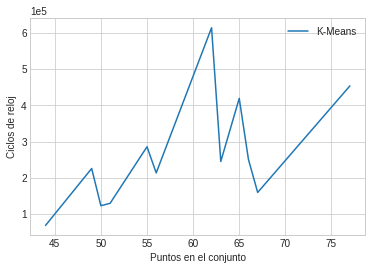
\includegraphics[scale=0.55]{exercise5/kmeans3}
	\end{minipage}\qquad
	\begin{minipage}[t]{.45\textwidth}
		\centering
		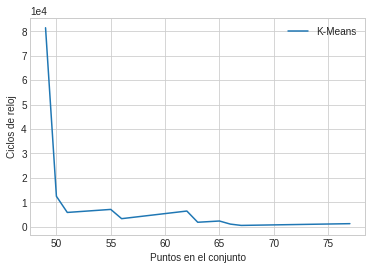
\includegraphics[scale=0.55]{exercise5/kmeansAcotado}
	\end{minipage}
\end{figure}

Tal como era de esperar, el gráfico no presenta una curva de crecimiento continuo a medida que crece el valor de n. Sin embargo, en el gráfico de la derecha vemos como la curva que representa a los puntos del gráfico del lado izquierdo, divididos por la cota de complejidad temporal, converge. Esto muestra que la heurística respeta la complejidad temproal planteada.

Luego, podemos concluir que la distribución de los puntos afecta en gran parte a la performance del algoritmo.


\subsubsubsection{Medición en base a distribución del grafo}

Dado que este algoritmo se comporta mejor en casos con clusters, se decidió comparar un caso de clusters contra otro generado aleatoriamente. Se espera que el caso generado con clusters sea más rápido.

\begin{figure}[H]
	\centering
	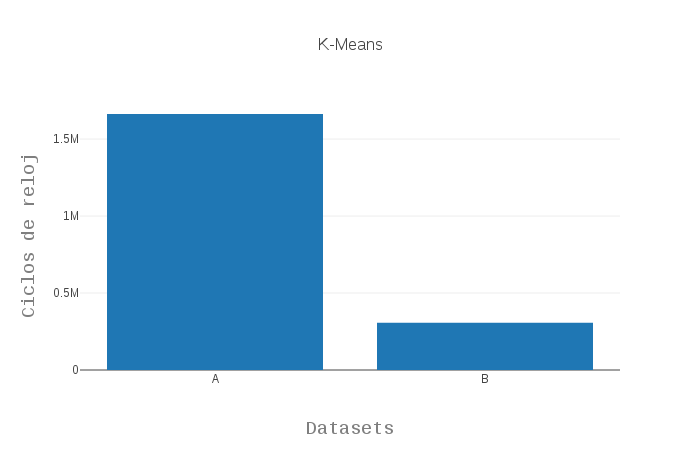
\includegraphics[scale=0.4]{exercise5/kmeansType.png}
\end{figure}

El gráfico cumple con la suposición.
\subsubsection{Heurística constructiva de cluster-first, route-second, clusterizando con algoritmo de K-means}

\subsubsubsection{Medición en base a tamaño del grafo}

En este caso, la heurística plantea que en peor caso tendremos k clusters igual a n, con una complejidad temporal de $\mathcal{O}(n^{2} * log(n))$. Es por ello que en algunos casos podemos tener k clusters menores a n, por ello, es de esperar un gráfico con variaciones.

\begin{figure}[H]
	\centering
	\begin{minipage}[t]{.45\textwidth}
		\centering
		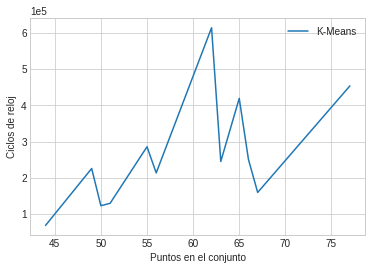
\includegraphics[scale=0.55]{exercise5/kmeans3}
	\end{minipage}\qquad
	\begin{minipage}[t]{.45\textwidth}
		\centering
		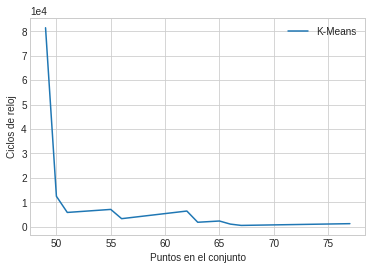
\includegraphics[scale=0.55]{exercise5/kmeansAcotado}
	\end{minipage}
\end{figure}

Tal como era de esperar, el gráfico no presenta una curva de crecimiento continuo a medida que crece el valor de n. Sin embargo, en el gráfico de la derecha vemos como la curva que representa a los puntos del gráfico del lado izquierdo, divididos por la cota de complejidad temporal, converge. Esto muestra que la heurística respeta la complejidad temproal planteada.

Luego, podemos concluir que la distribución de los puntos afecta en gran parte a la performance del algoritmo.


\subsubsubsection{Medición en base a distribución del grafo}

Dado que este algoritmo se comporta mejor en casos con clusters, se decidió comparar un caso de clusters contra otro generado aleatoriamente. Se espera que el caso generado con clusters sea más rápido.

\begin{figure}[H]
	\centering
	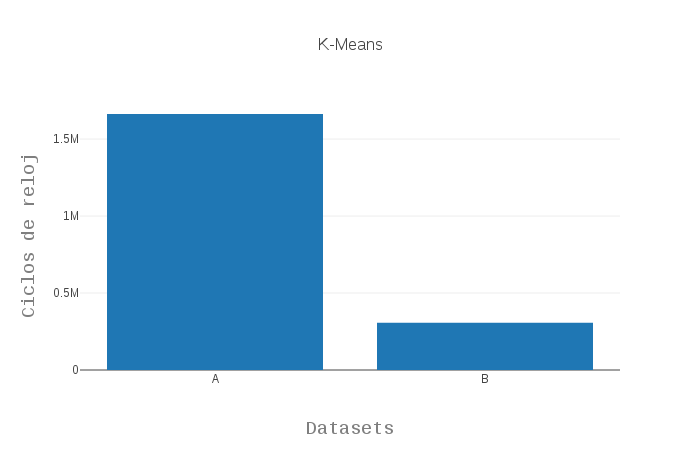
\includegraphics[scale=0.4]{exercise5/kmeansType.png}
\end{figure}

El gráfico cumple con la suposición.
\subsubsection{Heurística constructiva de cluster-first, route-second, clusterizando con algoritmo de K-means}

\subsubsubsection{Medición en base a tamaño del grafo}

En este caso, la heurística plantea que en peor caso tendremos k clusters igual a n, con una complejidad temporal de $\mathcal{O}(n^{2} * log(n))$. Es por ello que en algunos casos podemos tener k clusters menores a n, por ello, es de esperar un gráfico con variaciones.

\begin{figure}[H]
	\centering
	\begin{minipage}[t]{.45\textwidth}
		\centering
		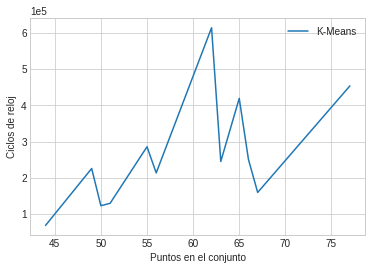
\includegraphics[scale=0.55]{exercise5/kmeans3}
	\end{minipage}\qquad
	\begin{minipage}[t]{.45\textwidth}
		\centering
		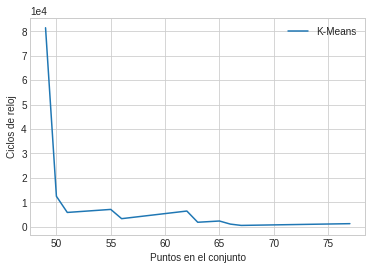
\includegraphics[scale=0.55]{exercise5/kmeansAcotado}
	\end{minipage}
\end{figure}

Tal como era de esperar, el gráfico no presenta una curva de crecimiento continuo a medida que crece el valor de n. Sin embargo, en el gráfico de la derecha vemos como la curva que representa a los puntos del gráfico del lado izquierdo, divididos por la cota de complejidad temporal, converge. Esto muestra que la heurística respeta la complejidad temproal planteada.

Luego, podemos concluir que la distribución de los puntos afecta en gran parte a la performance del algoritmo.


\subsubsubsection{Medición en base a distribución del grafo}

Dado que este algoritmo se comporta mejor en casos con clusters, se decidió comparar un caso de clusters contra otro generado aleatoriamente. Se espera que el caso generado con clusters sea más rápido.

\begin{figure}[H]
	\centering
	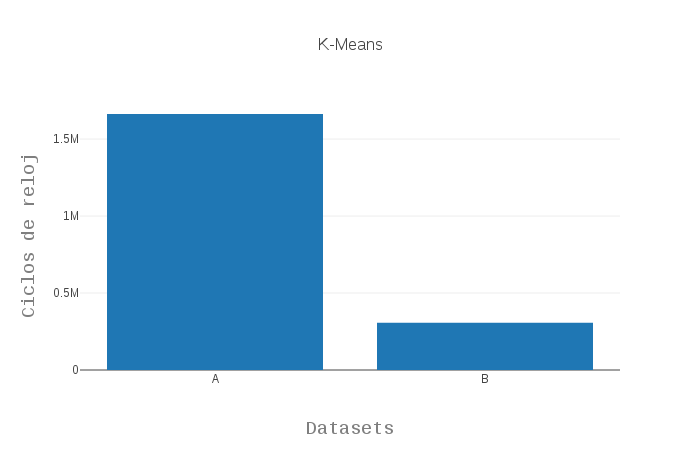
\includegraphics[scale=0.4]{exercise5/kmeansType.png}
\end{figure}

El gráfico cumple con la suposición.
\subsubsection{Heurística constructiva de cluster-first, route-second, clusterizando con algoritmo de K-means}

\subsubsubsection{Medición en base a tamaño del grafo}

En este caso, la heurística plantea que en peor caso tendremos k clusters igual a n, con una complejidad temporal de $\mathcal{O}(n^{2} * log(n))$. Es por ello que en algunos casos podemos tener k clusters menores a n, por ello, es de esperar un gráfico con variaciones.

\begin{figure}[H]
	\centering
	\begin{minipage}[t]{.45\textwidth}
		\centering
		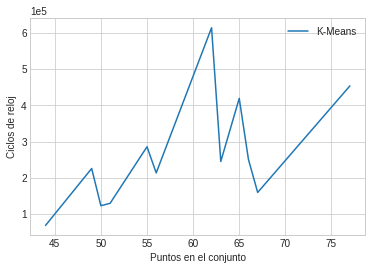
\includegraphics[scale=0.55]{exercise5/kmeans3}
	\end{minipage}\qquad
	\begin{minipage}[t]{.45\textwidth}
		\centering
		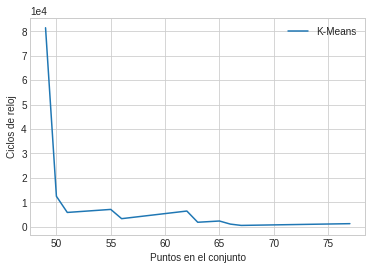
\includegraphics[scale=0.55]{exercise5/kmeansAcotado}
	\end{minipage}
\end{figure}

Tal como era de esperar, el gráfico no presenta una curva de crecimiento continuo a medida que crece el valor de n. Sin embargo, en el gráfico de la derecha vemos como la curva que representa a los puntos del gráfico del lado izquierdo, divididos por la cota de complejidad temporal, converge. Esto muestra que la heurística respeta la complejidad temproal planteada.

Luego, podemos concluir que la distribución de los puntos afecta en gran parte a la performance del algoritmo.


\subsubsubsection{Medición en base a distribución del grafo}

Dado que este algoritmo se comporta mejor en casos con clusters, se decidió comparar un caso de clusters contra otro generado aleatoriamente. Se espera que el caso generado con clusters sea más rápido.

\begin{figure}[H]
	\centering
	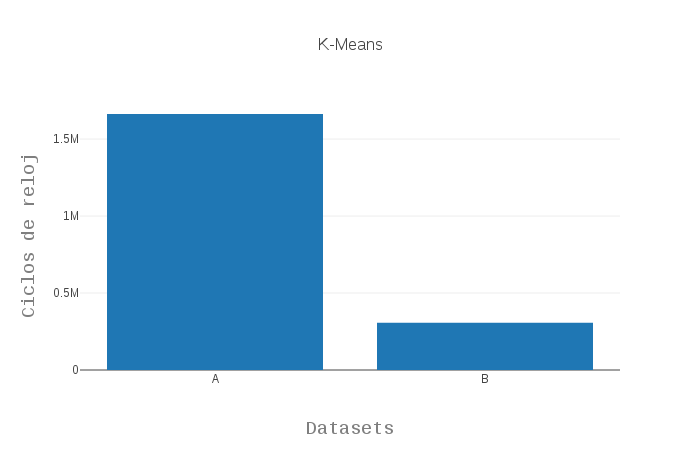
\includegraphics[scale=0.4]{exercise5/kmeansType.png}
\end{figure}

El gráfico cumple con la suposición.
\subsubsection{Heurística constructiva de cluster-first, route-second, clusterizando con algoritmo de K-means}

\subsubsubsection{Medición en base a tamaño del grafo}

En este caso, la heurística plantea que en peor caso tendremos k clusters igual a n, con una complejidad temporal de $\mathcal{O}(n^{2} * log(n))$. Es por ello que en algunos casos podemos tener k clusters menores a n, por ello, es de esperar un gráfico con variaciones.

\begin{figure}[H]
	\centering
	\begin{minipage}[t]{.45\textwidth}
		\centering
		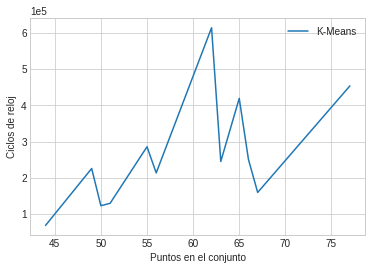
\includegraphics[scale=0.55]{exercise5/kmeans3}
	\end{minipage}\qquad
	\begin{minipage}[t]{.45\textwidth}
		\centering
		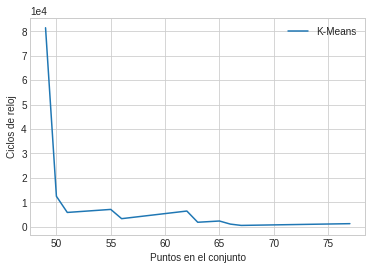
\includegraphics[scale=0.55]{exercise5/kmeansAcotado}
	\end{minipage}
\end{figure}

Tal como era de esperar, el gráfico no presenta una curva de crecimiento continuo a medida que crece el valor de n. Sin embargo, en el gráfico de la derecha vemos como la curva que representa a los puntos del gráfico del lado izquierdo, divididos por la cota de complejidad temporal, converge. Esto muestra que la heurística respeta la complejidad temproal planteada.

Luego, podemos concluir que la distribución de los puntos afecta en gran parte a la performance del algoritmo.


\subsubsubsection{Medición en base a distribución del grafo}

Dado que este algoritmo se comporta mejor en casos con clusters, se decidió comparar un caso de clusters contra otro generado aleatoriamente. Se espera que el caso generado con clusters sea más rápido.

\begin{figure}[H]
	\centering
	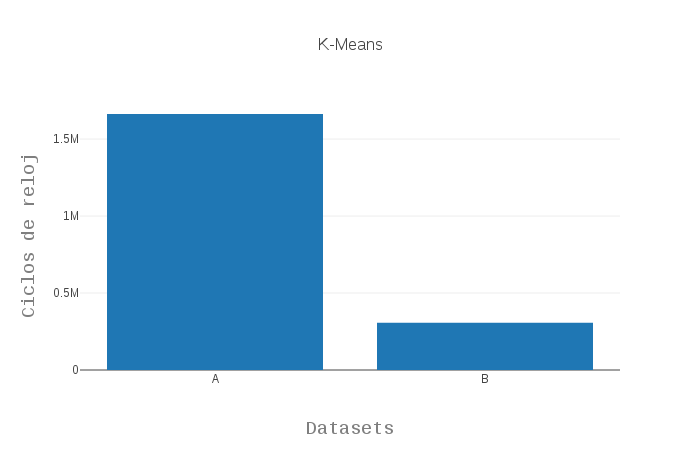
\includegraphics[scale=0.4]{exercise5/kmeansType.png}
\end{figure}

El gráfico cumple con la suposición.

\subsubsection{Conclusiones}
 A la hora de resolver el problema de Enrutamiento de Vehículos con Capacidad disponemos de innumerables heurísticas y algoritmos para aproximarnos a la solución más óptima en el tiempo disponible. Algunas de estas son rápidas y otras no tanto. En este documento, las más veloces aún tienen chances de competir con las más robustas en algunos casos puntuales. Esto motivó a evaluar en qué casos podríamos aprovechar la simplicidad y reducido costo temporal de estas heurísticas versus aquellas más demandantes sin perder calidad en nuestras soluciones, pero todavía no nos hemos respondido una pregunta fundamental: ¿Cuál es la mejor heurística? Esta pregunta – así formulada – no tiene respuesta, pues depende de cuántos vértices componen nuestra instancia del problema, cómo es su distribución, cuáles son sus demandas, etcétera. Tal vez, reformulando la pregunta, podemos llegar a una respuesta: en los datasets disponibles para este trabajo, ¿cuál es el algoritmo que, en promedio, minimiza mejor las distancias recorridas? Averiguemoslo:

 \begin{figure}[H]
 	\centering
	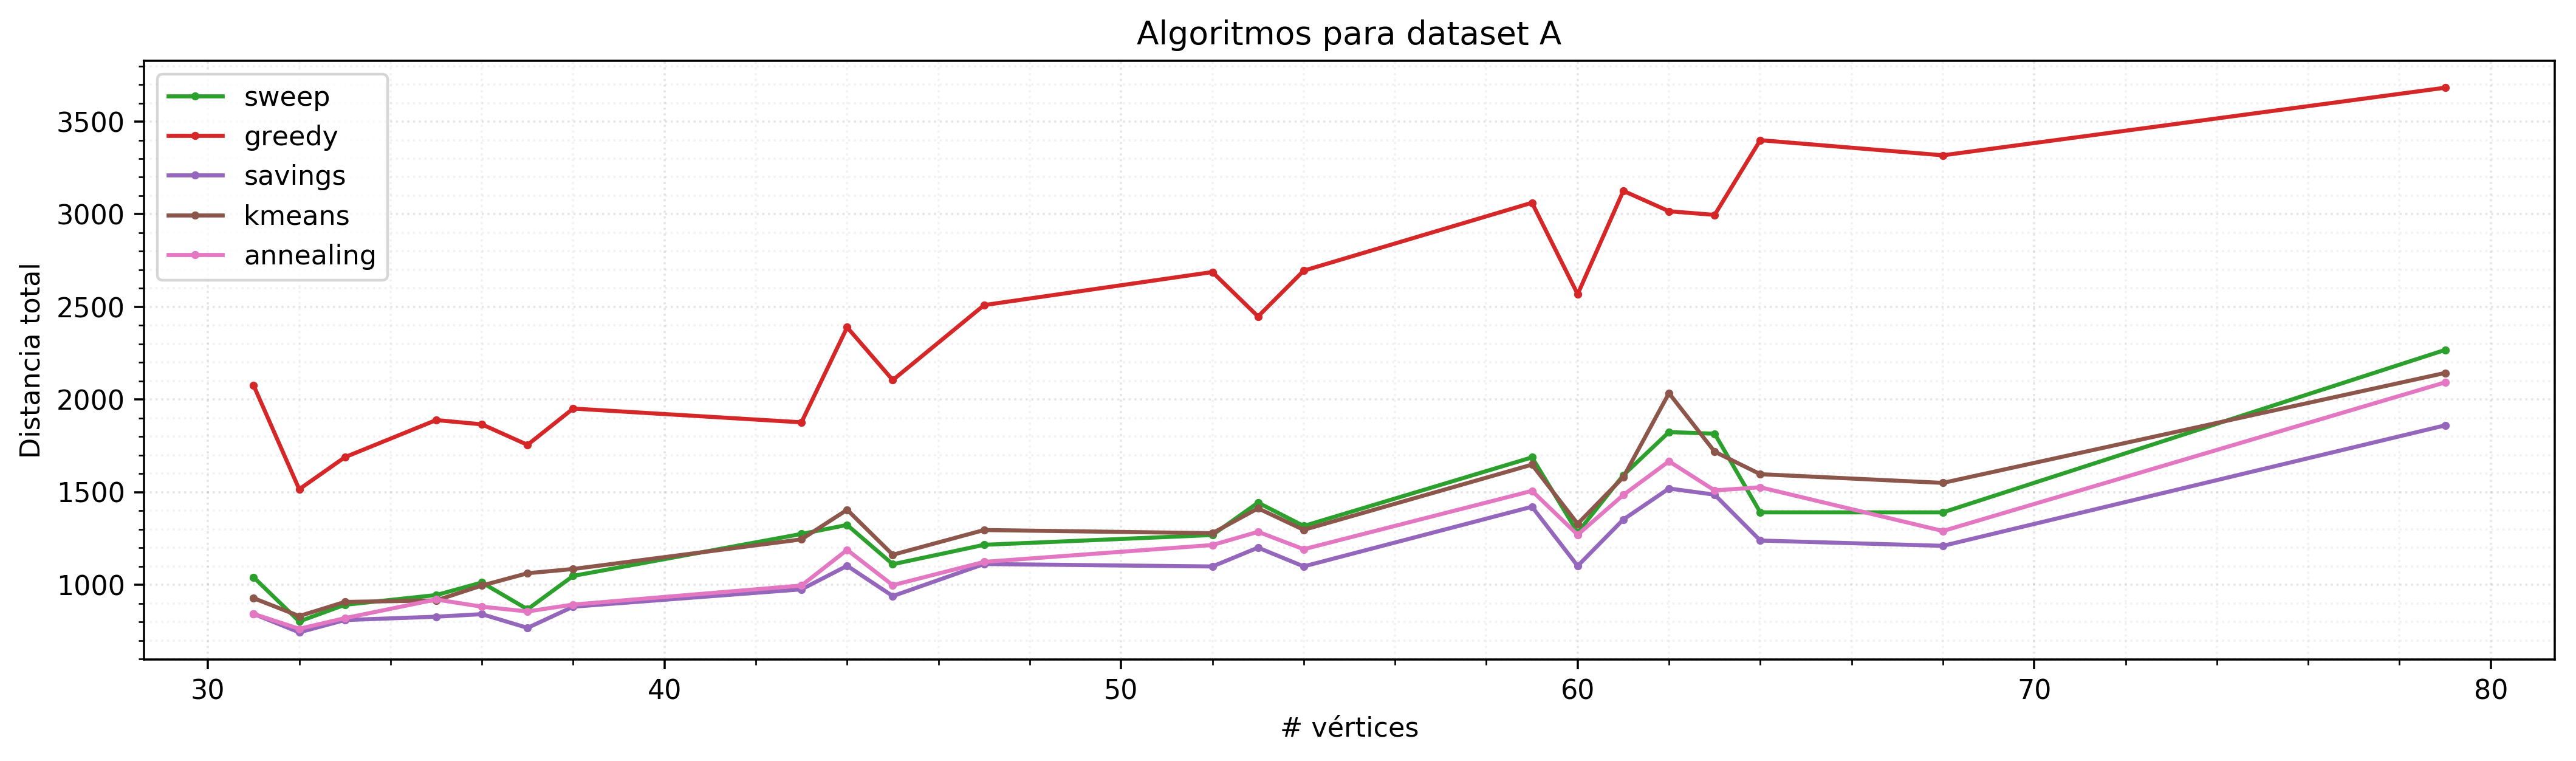
\includegraphics[width=1\textwidth]{algorithms-distances-for-A}
	\caption{\footnotesize Promedio de distancias totales para cada algoritmo resolviendo todas las instancias del dataset \textbf{A}, generadas con vértices al azar, capacidad $=100$, demanda promedio $=15$.}
	\label{fig:algorithms-distances-for-A}
 \end{figure}

Las tendencias son visibles. Podemos concluir que la heurística golosa constructiva no tiene un buen desempeño en casos estocásticos, donde los puntos están distribuidos de manera aleatoria al rededor del depósito. Esta heurística puede otorgar soluciones hasta dos veces peores que cualquier otra heurística y a menos que estemos hablando de casos particulares, no creemos que valga la pena considerar esta técnica para resolver instancias de CVRP de estas características. Con respecto al resto de los algoritmos, las soluciones de \textbf{Savings} se imponen por sobre el resto en todos los casos. De cerca le sigue \textbf{Annealing} y alternándose entre uno y otro compiten \textbf{K-Means} y \textbf{Sweep}. Observemos el desempeño de los algoritmos para otro dataset:

\begin{figure}[H]
 \centering
 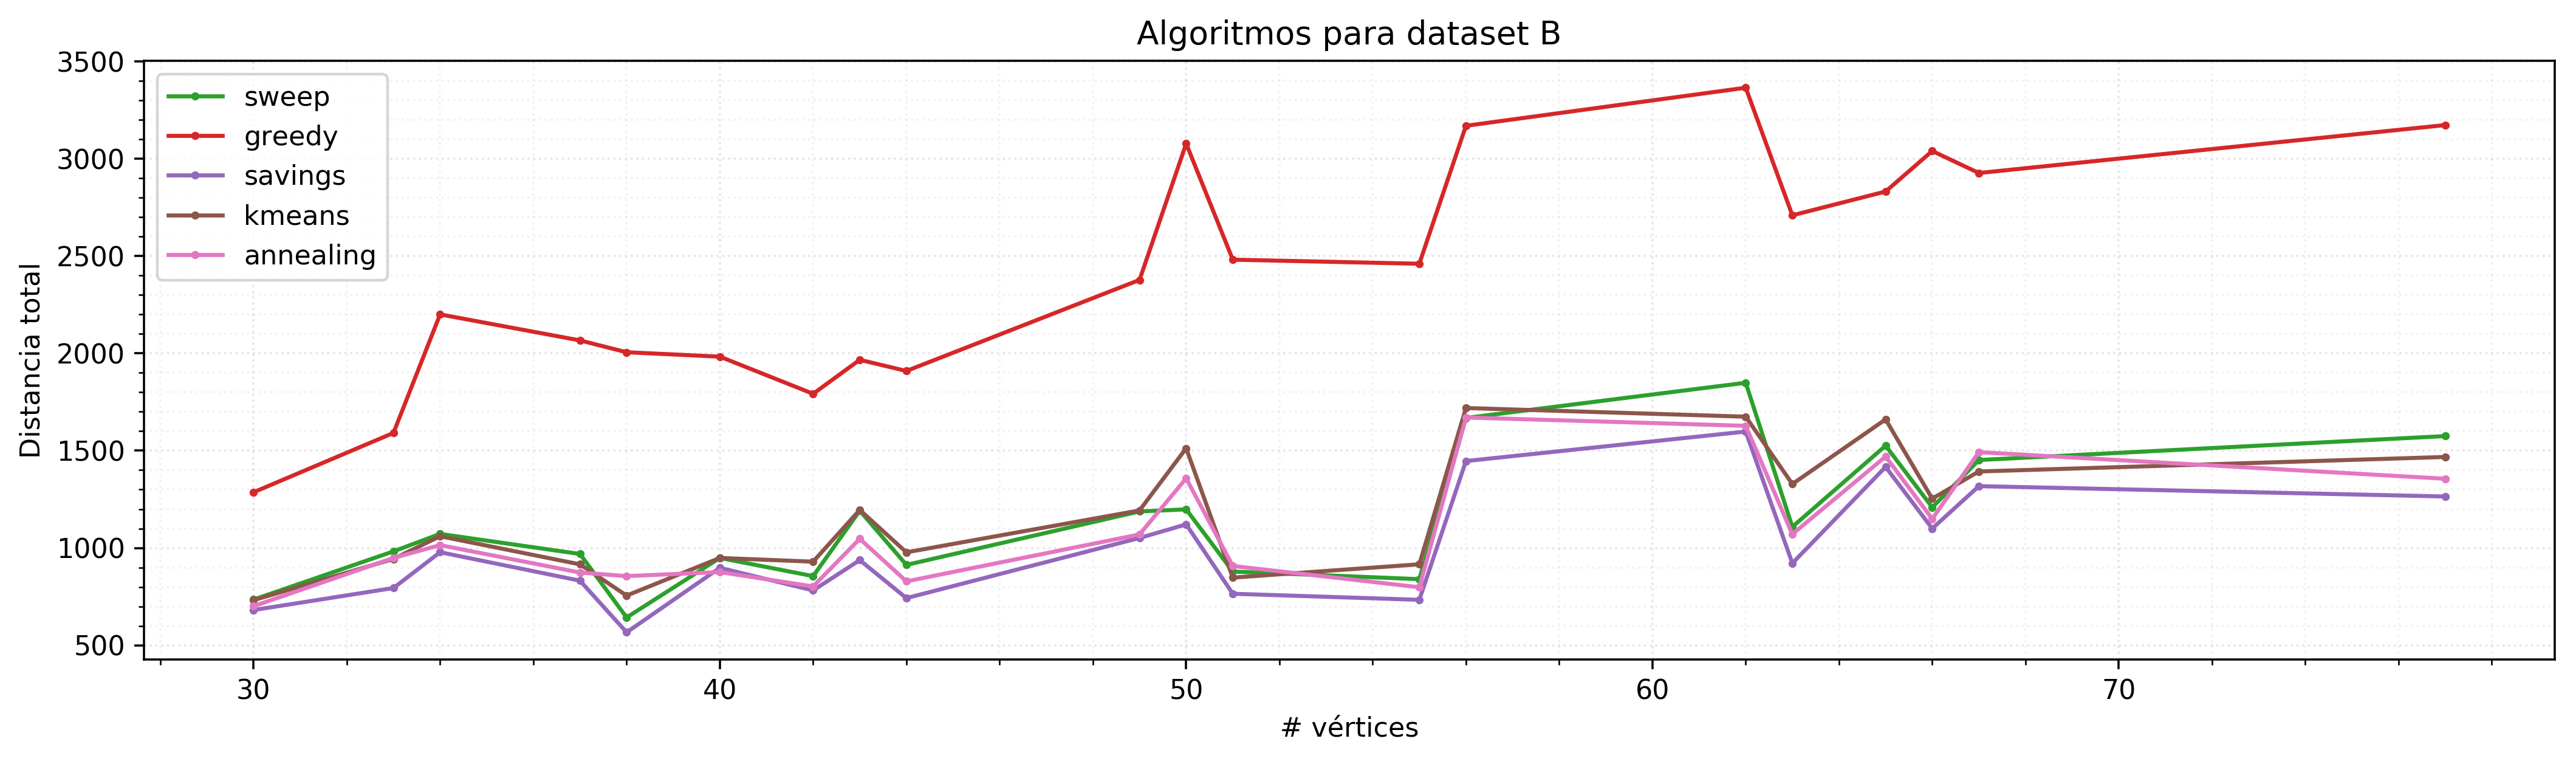
\includegraphics[width=1\textwidth]{algorithms-distances-for-B}
 \caption{\footnotesize Promedio de distancias totales para cada algoritmo resolviendo todas las instancias del dataset \textbf{B} donde los clientes pertenecen a clusters bien definidos.}
 \label{fig:algorithms-distances-for-B}
\end{figure}

Aquí, la tendencia con respecto al algoritmo goloso remanece, quien sigue siendo la peor opción. Por otro lado, el resto de los algoritmos parece coincidir aproximadamente en la calidad de las soluciones. Hay que resaltar que este dataset distribuye los vértices en clusters naturales, por lo cual heurísticas como \textbf{K-Means} y \textbf{Sweep} tienen un mejor desempeño – y en consecuencia están más cerca a las soluciones de \textbf{Annealing} y \textbf{Savings} – que en el dataset anterior, donde la aleatoreidad de la posición de los clientes dificulta el proceso de clusterización. Observemos este comportamiento en más detalle removiendo a \textbf{Greedy} del panorama:

\begin{figure}[H]
	\centering
	\begin{minipage}{0.48\textwidth}
		\centering
		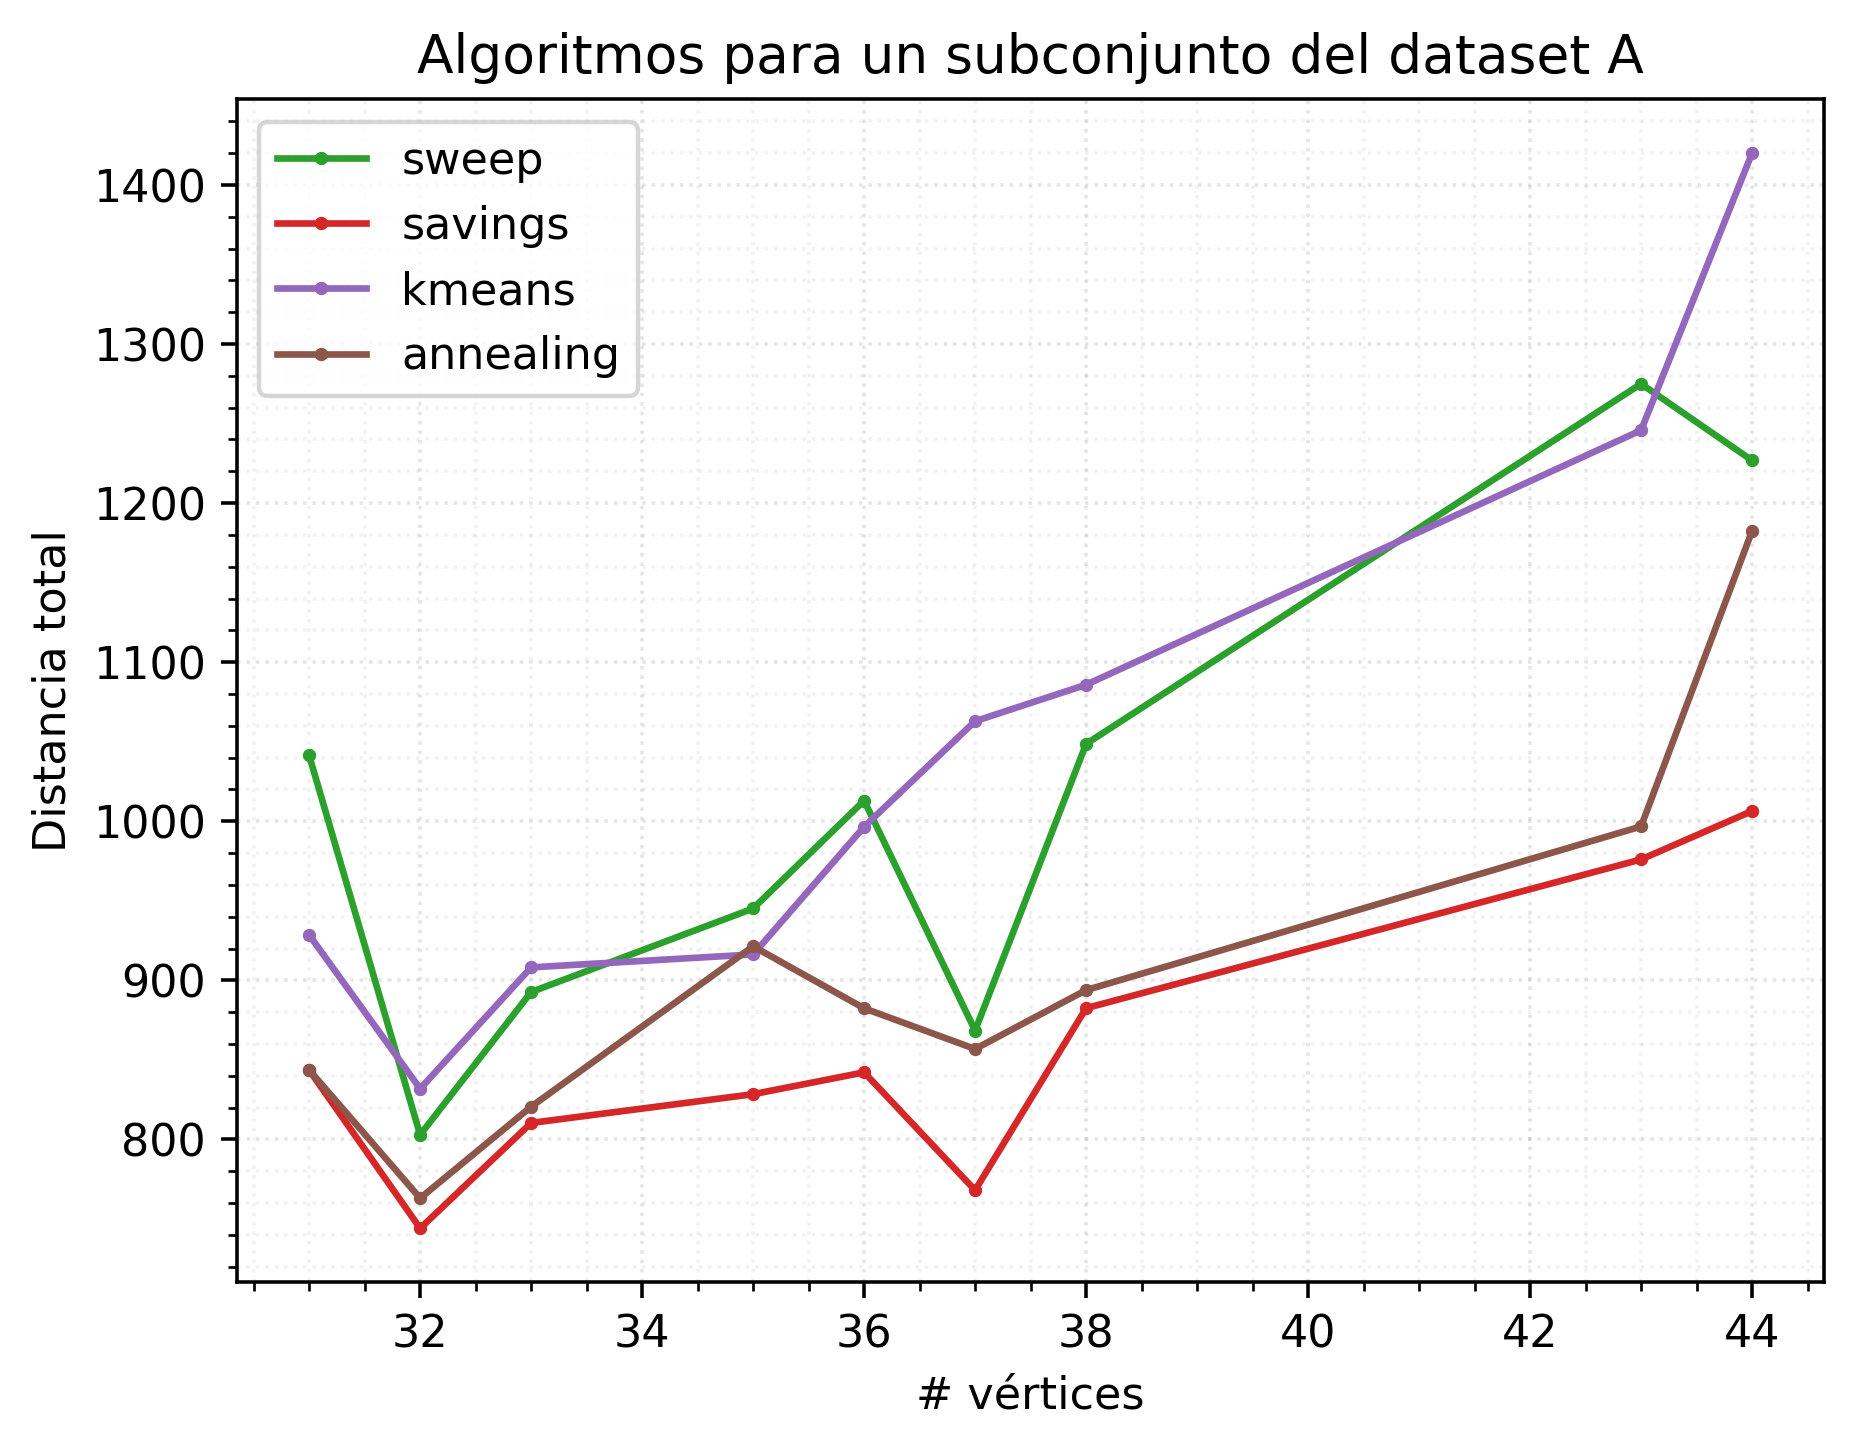
\includegraphics[width=1\textwidth]{algorithms-distances-for-A-nogr}
		\caption{\footnotesize Solución golosa constructiva quasi-óptima.}
		\label{fig:algorithms-distances-for-A-nogr}
	\end{minipage}%
	\hspace{0.03\textwidth}
	\begin{minipage}{0.48\textwidth}
		\centering
		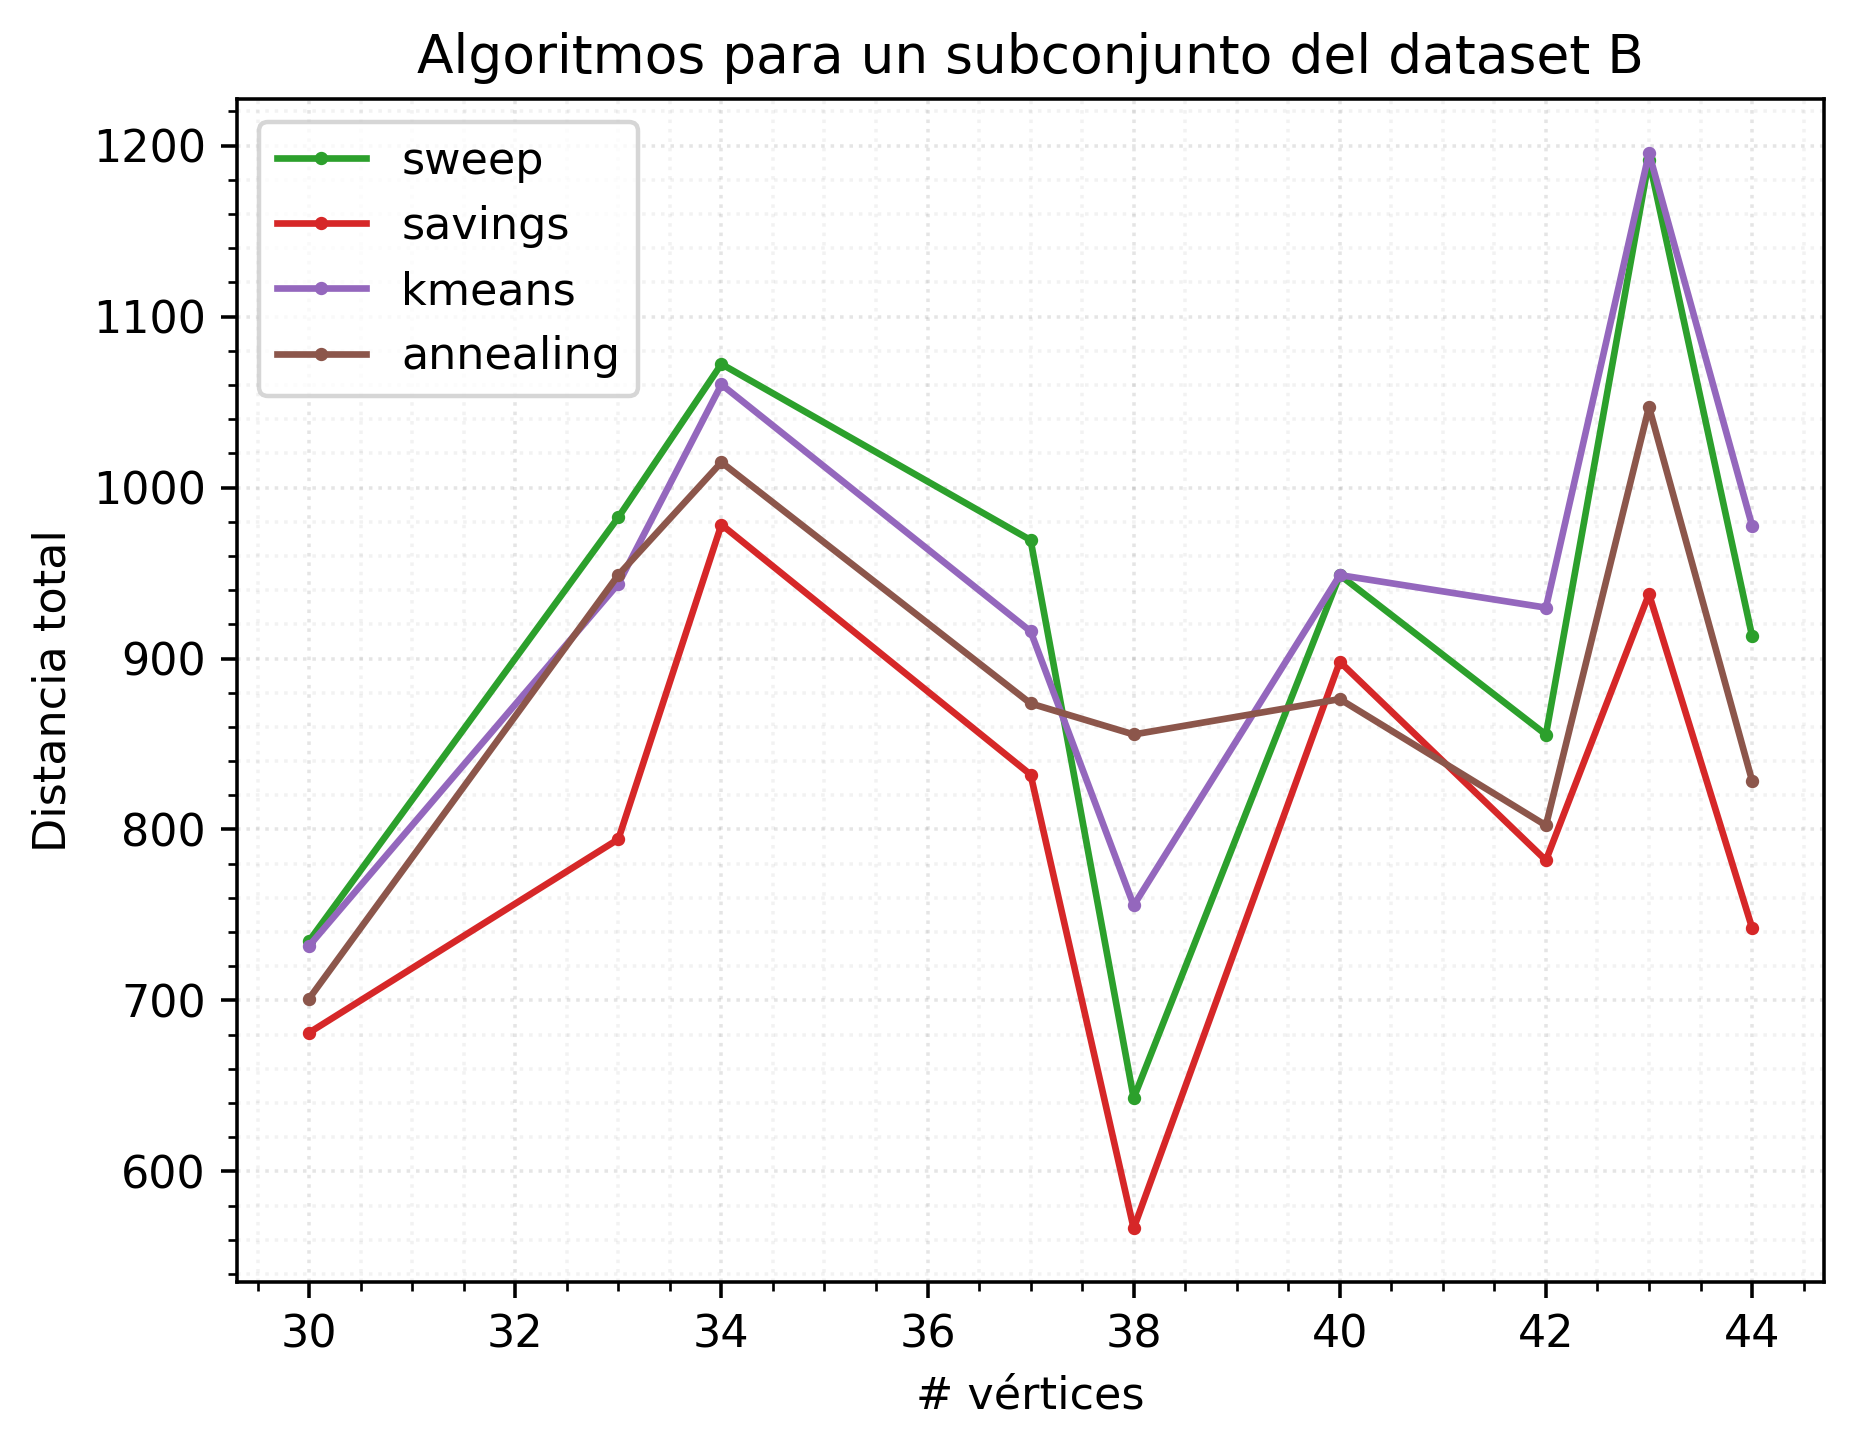
\includegraphics[width=1\textwidth]{algorithms-distances-for-B-nogr}
		\caption{\footnotesize Solución óptima con \textbf{savings}.}
		\label{fig:algorithms-distances-for-B-nogr}
	\end{minipage}%
\end{figure}

Podemos observar que, si bien cada gráfico representa soluciones a instancias distintas, uno muestra a \textbf{Sweep} y \textbf{K-Means} mucho más cerca a \textbf{Annealing} y \textbf{Savings} que el otro, como fue explicado anteriormente. Sin embargo, en todos estos análisis \textbf{Savings} sigue siendo la opción superadora para cualquier instancia del problema del cual, a priori, no se sabe nada.
